\chapter{Ghosts}

At first sight, the exterior of the house at Auteuil gave no
indications of splendor, nothing one would expect from the destined
residence of the magnificent Count of Monte Cristo; but this simplicity
was according to the will of its master, who positively ordered nothing
to be altered outside. The splendor was within. Indeed, almost before
the door opened, the scene changed.

M. Bertuccio had outdone himself in the taste displayed in furnishing,
and in the rapidity with which it was executed. It is told that the Duc
d’Antin removed in a single night a whole avenue of trees that annoyed
Louis XIV.; in three days M. Bertuccio planted an entirely bare court
with poplars, large spreading sycamores to shade the different parts of
the house, and in the foreground, instead of the usual paving-stones,
half hidden by the grass, there extended a lawn but that morning laid
down, and upon which the water was yet glistening. For the rest, the
orders had been issued by the count; he himself had given a plan to
Bertuccio, marking the spot where each tree was to be planted, and the
shape and extent of the lawn which was to take the place of the
paving-stones.

Thus the house had become unrecognizable, and Bertuccio himself
declared that he scarcely knew it, encircled as it was by a framework
of trees. The overseer would not have objected, while he was about it,
to have made some improvements in the garden, but the count had
positively forbidden it to be touched. Bertuccio made amends, however,
by loading the antechambers, staircases, and mantle-pieces with
flowers.

What, above all, manifested the shrewdness of the steward, and the
profound science of the master, the one in carrying out the ideas of
the other, was that this house which appeared only the night before so
sad and gloomy, impregnated with that sickly smell one can almost fancy
to be the smell of time, had in a single day acquired the aspect of
life, was scented with its master’s favorite perfumes, and had the very
light regulated according to his wish. When the count arrived, he had
under his touch his books and arms, his eyes rested upon his favorite
pictures; his dogs, whose caresses he loved, welcomed him in the
antechamber; the birds, whose songs delighted him, cheered him with
their music; and the house, awakened from its long sleep, like the
sleeping beauty in the wood, lived, sang, and bloomed like the houses
we have long cherished, and in which, when we are forced to leave them,
we leave a part of our souls.

The servants passed gayly along the fine courtyard; some, belonging to
the kitchens, gliding down the stairs, restored but the previous day,
as if they had always inhabited the house; others filling the
coach-houses, where the equipages, encased and numbered, appeared to
have been installed for the last fifty years; and in the stables the
horses replied with neighs to the grooms, who spoke to them with much
more respect than many servants pay their masters.

The library was divided into two parts on either side of the wall, and
contained upwards of two thousand volumes; one division was entirely
devoted to novels, and even the volume which had been published but the
day before was to be seen in its place in all the dignity of its red
and gold binding.

On the other side of the house, to match with the library, was the
conservatory, ornamented with rare flowers, that bloomed in china jars;
and in the midst of the greenhouse, marvellous alike to sight and
smell, was a billiard-table which looked as if it had been abandoned
during the past hour by players who had left the balls on the cloth.

One chamber alone had been respected by the magnificent Bertuccio.
Before this room, to which you could ascend by the grand, and go out by
the back staircase, the servants passed with curiosity, and Bertuccio
with terror.

At five o’clock precisely, the count arrived before the house at
Auteuil, followed by Ali. Bertuccio was awaiting this arrival with
impatience, mingled with uneasiness; he hoped for some compliments,
while, at the same time, he feared to have frowns. Monte Cristo
descended into the courtyard, walked all over the house, without giving
any sign of approbation or pleasure, until he entered his bedroom,
situated on the opposite side to the closed room; then he approached a
little piece of furniture, made of rosewood, which he had noticed at a
previous visit.

“That can only be to hold gloves,” he said.

“Will your excellency deign to open it?” said the delighted Bertuccio,
“and you will find gloves in it.”

Elsewhere the count found everything he required—smelling-bottles,
cigars, knick-knacks.

\begin{figure}[ht]
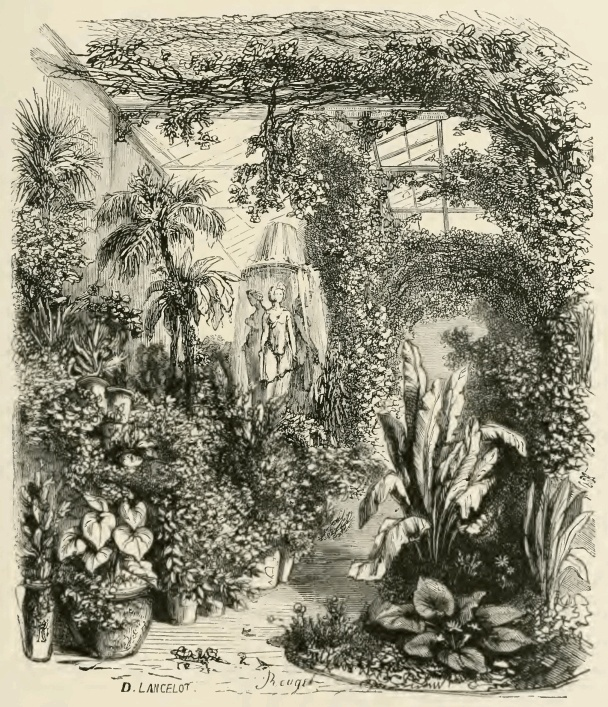
\includegraphics[width=\textwidth]{30207m.jpg}
\end{figure}

“Good,” he said; and M. Bertuccio left enraptured, so great, so
powerful, and real was the influence exercised by this man over all who
surrounded him.

At precisely six o’clock the clatter of horses’ hoofs was heard at the
entrance door; it was our captain of Spahis, who had arrived on Médéah.
“I am sure I am the first,” cried Morrel; “I did it on purpose to have
you a minute to myself, before everyone came. Julie and Emmanuel have a
thousand things to tell you. Ah, really this is magnificent! But tell
me, count, will your people take care of my horse?”

“Do not alarm yourself, my dear Maximilian—they understand.”

“I mean, because he wants petting. If you had seen at what a pace he
came—like the wind!”

“I should think so,—a horse that cost 5,000 francs!” said Monte Cristo,
in the tone which a father would use towards a son.

“Do you regret them?” asked Morrel, with his open laugh.

“I? Certainly not,” replied the count. “No; I should only regret if the
horse had not proved good.”

“It is so good, that I have distanced M. de Château-Renaud, one of the
best riders in France, and M. Debray, who both mount the minister’s
Arabians; and close on their heels are the horses of Madame Danglars,
who always go at six leagues an hour.”

“Then they follow you?” asked Monte Cristo.

“See, they are here.” And at the same minute a carriage with smoking
horses, accompanied by two mounted gentlemen, arrived at the gate,
which opened before them. The carriage drove round, and stopped at the
steps, followed by the horsemen.

The instant Debray had touched the ground, he was at the carriage-door.
He offered his hand to the baroness, who, descending, took it with a
peculiarity of manner imperceptible to everyone but Monte Cristo. But
nothing escaped the count’s notice, and he observed a little note,
passed with the facility that indicates frequent practice, from the
hand of Madame Danglars to that of the minister’s secretary.

After his wife the banker descended, as pale as though he had issued
from his tomb instead of his carriage.

Madame Danglars threw a rapid and inquiring glance which could only be
interpreted by Monte Cristo, around the courtyard, over the peristyle,
and across the front of the house, then, repressing a slight emotion,
which must have been seen on her countenance if she had not kept her
color, she ascended the steps, saying to Morrel:

“Sir, if you were a friend of mine, I should ask you if you would sell
your horse.”

Morrel smiled with an expression very like a grimace, and then turned
round to Monte Cristo, as if to ask him to extricate him from his
embarrassment. The count understood him.

“Ah, madame,” he said, “why did you not make that request of me?”

“With you, sir,” replied the baroness, “one can wish for nothing, one
is so sure to obtain it. If it were so with M. Morrel——”

“Unfortunately,” replied the count, “I am witness that M. Morrel cannot
give up his horse, his honor being engaged in keeping it.”

“How so?”

“He laid a wager he would tame Médéah in the space of six months. You
understand now that if he were to get rid of the animal before the time
named, he would not only lose his bet, but people would say he was
afraid; and a brave captain of Spahis cannot risk this, even to gratify
a pretty woman, which is, in my opinion, one of the most sacred
obligations in the world.”

“You see my position, madame,” said Morrel, bestowing a grateful smile
on Monte Cristo.

“It seems to me,” said Danglars, in his coarse tone, ill-concealed by a
forced smile, “that you have already got horses enough.”

Madame Danglars seldom allowed remarks of this kind to pass unnoticed,
but, to the surprise of the young people, she pretended not to hear it,
and said nothing. Monte Cristo smiled at her unusual humility, and
showed her two immense porcelain jars, over which wound marine plants,
of a size and delicacy that nature alone could produce. The baroness
was astonished.

“Why,” said she, “you could plant one of the chestnut-trees in the
Tuileries inside! How can such enormous jars have been manufactured?”

“Ah! madame,” replied Monte Cristo, “you must not ask of us, the
manufacturers of fine porcelain, such a question. It is the work of
another age, constructed by the genii of earth and water.”

“How so?—at what period can that have been?”

“I do not know; I have only heard that an emperor of China had an oven
built expressly, and that in this oven twelve jars like this were
successively baked. Two broke, from the heat of the fire; the other ten
were sunk three hundred fathoms deep into the sea. The sea, knowing
what was required of her, threw over them her weeds, encircled them
with coral, and encrusted them with shells; the whole was cemented by
two hundred years beneath these almost impervious depths, for a
revolution carried away the emperor who wished to make the trial, and
only left the documents proving the manufacture of the jars and their
descent into the sea. At the end of two hundred years the documents
were found, and they thought of bringing up the jars. Divers descended
in machines, made expressly on the discovery, into the bay where they
were thrown; but of ten three only remained, the rest having been
broken by the waves. I am fond of these jars, upon which, perhaps,
misshapen, frightful monsters have fixed their cold, dull eyes, and in
which myriads of small fish have slept, seeking a refuge from the
pursuit of their enemies.”

Meanwhile, Danglars, who had cared little for curiosities, was
mechanically tearing off the blossoms of a splendid orange-tree, one
after another. When he had finished with the orange-tree, he began at
the cactus; but this, not being so easily plucked as the orange-tree,
pricked him dreadfully. He shuddered, and rubbed his eyes as though
awaking from a dream.

“Sir,” said Monte Cristo to him, “I do not recommend my pictures to
you, who possess such splendid paintings; but, nevertheless, here are
two by Hobbema, a Paul Potter, a Mieris, two by Gerard Douw, a Raphael,
a Van Dyck, a Zurbaran, and two or three by Murillo, worth looking at.”

“Stay,” said Debray; “I recognize this Hobbema.”

“Ah, indeed!”

“Yes; it was proposed for the Museum.”

“Which, I believe, does not contain one?” said Monte Cristo.

“No; and yet they refused to buy it.”

“Why?” said Château-Renaud.

“You pretend not to know,—because government was not rich enough.”

“Ah, pardon me,” said Château-Renaud; “I have heard of these things
every day during the last eight years, and I cannot understand them
yet.”

“You will, by and by,” said Debray.

“I think not,” replied Château-Renaud.

“Major Bartolomeo Cavalcanti and Count Andrea Cavalcanti,” announced
Baptistin.

A black satin stock, fresh from the maker’s hands, gray moustaches, a
bold eye, a major’s uniform, ornamented with three medals and five
crosses—in fact, the thorough bearing of an old soldier—such was the
appearance of Major Bartolomeo Cavalcanti, that tender father with whom
we are already acquainted. Close to him, dressed in entirely new
clothes, advanced smilingly Count Andrea Cavalcanti, the dutiful son,
whom we also know. The three young people were talking together. On the
entrance of the new-comers, their eyes glanced from father to son, and
then, naturally enough, rested on the latter, whom they began
criticising.

“Cavalcanti!” said Debray.

“A fine name,” said Morrel.

“Yes,” said Château-Renaud, “these Italians are well named and badly
dressed.”

“You are fastidious, Château-Renaud,” replied Debray; “those clothes
are well cut and quite new.”

“That is just what I find fault with. That gentleman appears to be well
dressed for the first time in his life.”

“Who are those gentlemen?” asked Danglars of Monte Cristo.

“You heard—Cavalcanti.”

“That tells me their name, and nothing else.”

“Ah! true. You do not know the Italian nobility; the Cavalcanti are all
descended from princes.”

“Have they any fortune?”

“An enormous one.”

“What do they do?”

“Try to spend it all. They have some business with you, I think, from
what they told me the day before yesterday. I, indeed, invited them
here today on your account. I will introduce you to them.”

“But they appear to speak French with a very pure accent,” said
Danglars.

“The son has been educated in a college in the south; I believe near
Marseilles. You will find him quite enthusiastic.”

“Upon what subject?” asked Madame Danglars.

“The French ladies, madame. He has made up his mind to take a wife from
Paris.”

“A fine idea that of his,” said Danglars, shrugging his shoulders.
Madame Danglars looked at her husband with an expression which, at any
other time, would have indicated a storm, but for the second time she
controlled herself.

“The baron appears thoughtful today,” said Monte Cristo to her; “are
they going to put him in the ministry?”

“Not yet, I think. More likely he has been speculating on the Bourse,
and has lost money.”

“M. and Madame de Villefort,” cried Baptistin.

They entered. M. de Villefort, notwithstanding his self-control, was
visibly affected, and when Monte Cristo touched his hand, he felt it
tremble.

“Certainly, women alone know how to dissimulate,” said Monte Cristo to
himself, glancing at Madame Danglars, who was smiling on the procureur,
and embracing his wife.

After a short time, the count saw Bertuccio, who, until then, had been
occupied on the other side of the house, glide into an adjoining room.
He went to him.

“What do you want, M. Bertuccio?” said he.

“Your excellency has not stated the number of guests.”

“Ah, true.”

“How many covers?”

“Count for yourself.”

“Is everyone here, your excellency?”

“Yes.”

Bertuccio glanced through the door, which was ajar. The count watched
him. “Good heavens!” he exclaimed.

“What is the matter?” said the count.

“That woman—that woman!”

“Which?”

“The one with a white dress and so many diamonds—the fair one.”

“Madame Danglars?”

“I do not know her name; but it is she, sir, it is she!”

“Whom do you mean?”

“The woman of the garden!—she that was \textit{enceinte}—she who was walking
while she waited for——”

Bertuccio stood at the open door, with his eyes starting and his hair
on end.

“Waiting for whom?” Bertuccio, without answering, pointed to Villefort
with something of the gesture Macbeth uses to point out Banquo.

“Oh, oh!” he at length muttered, “do you see?”

“What? Who?”

“Him!”

“Him!—M. de Villefort, the king’s attorney? Certainly I see him.”

“Then I did not kill him?”

“Really, I think you are going mad, good Bertuccio,” said the count.

“Then he is not dead?”

\begin{figure}[ht]
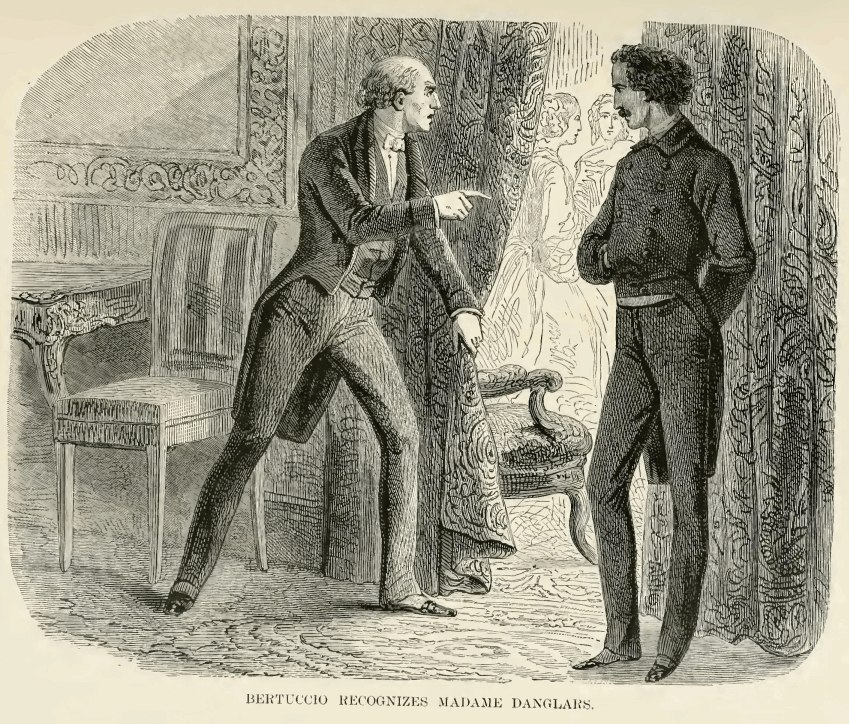
\includegraphics[width=\textwidth]{30213m.jpg}
\end{figure}

“No; you see plainly he is not dead. Instead of striking between the
sixth and seventh left ribs, as your countrymen do, you must have
struck higher or lower, and life is very tenacious in these lawyers, or
rather there is no truth in anything you have told me—it was a fright
of the imagination, a dream of your fancy. You went to sleep full of
thoughts of vengeance; they weighed heavily upon your stomach; you had
the nightmare—that’s all. Come, calm yourself, and reckon them up—M.
and Madame de Villefort, two; M. and Madame Danglars, four; M. de
Château-Renaud, M. Debray, M. Morrel, seven; Major Bartolomeo
Cavalcanti, eight.”

“Eight!” repeated Bertuccio.

“Stop! You are in a shocking hurry to be off—you forget one of my
guests. Lean a little to the left. Stay! look at M. Andrea Cavalcanti,
the young man in a black coat, looking at Murillo’s ‘Madonna’; now he
is turning.”

This time Bertuccio would have uttered an exclamation, had not a look
from Monte Cristo silenced him.

“Benedetto?” he muttered; “fatality!”

“Half-past six o’clock has just struck, M. Bertuccio,” said the count
severely; “I ordered dinner at that hour, and I do not like to wait;”
and he returned to his guests, while Bertuccio, leaning against the
wall, succeeded in reaching the dining-room. Five minutes afterwards
the doors of the drawing-room were thrown open, and Bertuccio appearing
said, with a violent effort, “The dinner waits.”

The Count of Monte Cristo offered his arm to Madame de Villefort. “M.
de Villefort,” he said, “will you conduct the Baroness Danglars?”

Villefort complied, and they passed on to the dining-room.
